\section{Introduction}
\label{sec:intro}

Deep learning in 3D medical imaging (CT, MRI, PET, SPECT) promises automated, high-precision clinical decision support~\cite{van2016convolutional, korkinof2018high}. However, transitioning algorithms from controlled single-center studies to heterogeneous multi-hospital environments reveals severe vulnerabilities~\cite{glocker2019machine, kamnitsas2017unsupervised}.

In multi-center clinical trials, scans are acquired across different hospital sites using diverse scanner vendors, magnetic field strengths, detector geometries, and voxel resolutions. Consequently, standard machine learning pipelines frequently learn \emph{scanner-specific background signatures} rather than true physiological disease biomarkers~\cite{subbanna2021review, dou2019domain}. A prevalent symptom of this vulnerability is \textbf{scanner-site data leakage}: when naive random or stratified cross-validation splits scans from the same scanner vendor or site across training and validation folds, validation metrics become artificially inflated ($\text{AUROC} > 0.98$), only to fail when evaluated on unseen clinical scanners.

Furthermore, medical classification models must produce well-calibrated posterior probabilities for downstream risk stratification~\cite{guo2017calibration}. Uncalibrated deep networks often exhibit severe overconfidence, assigning near-certain probability predictions ($p > 0.99$) even when incorrect, which compromises clinical utility.

\begin{figure}[t]
    \centering
    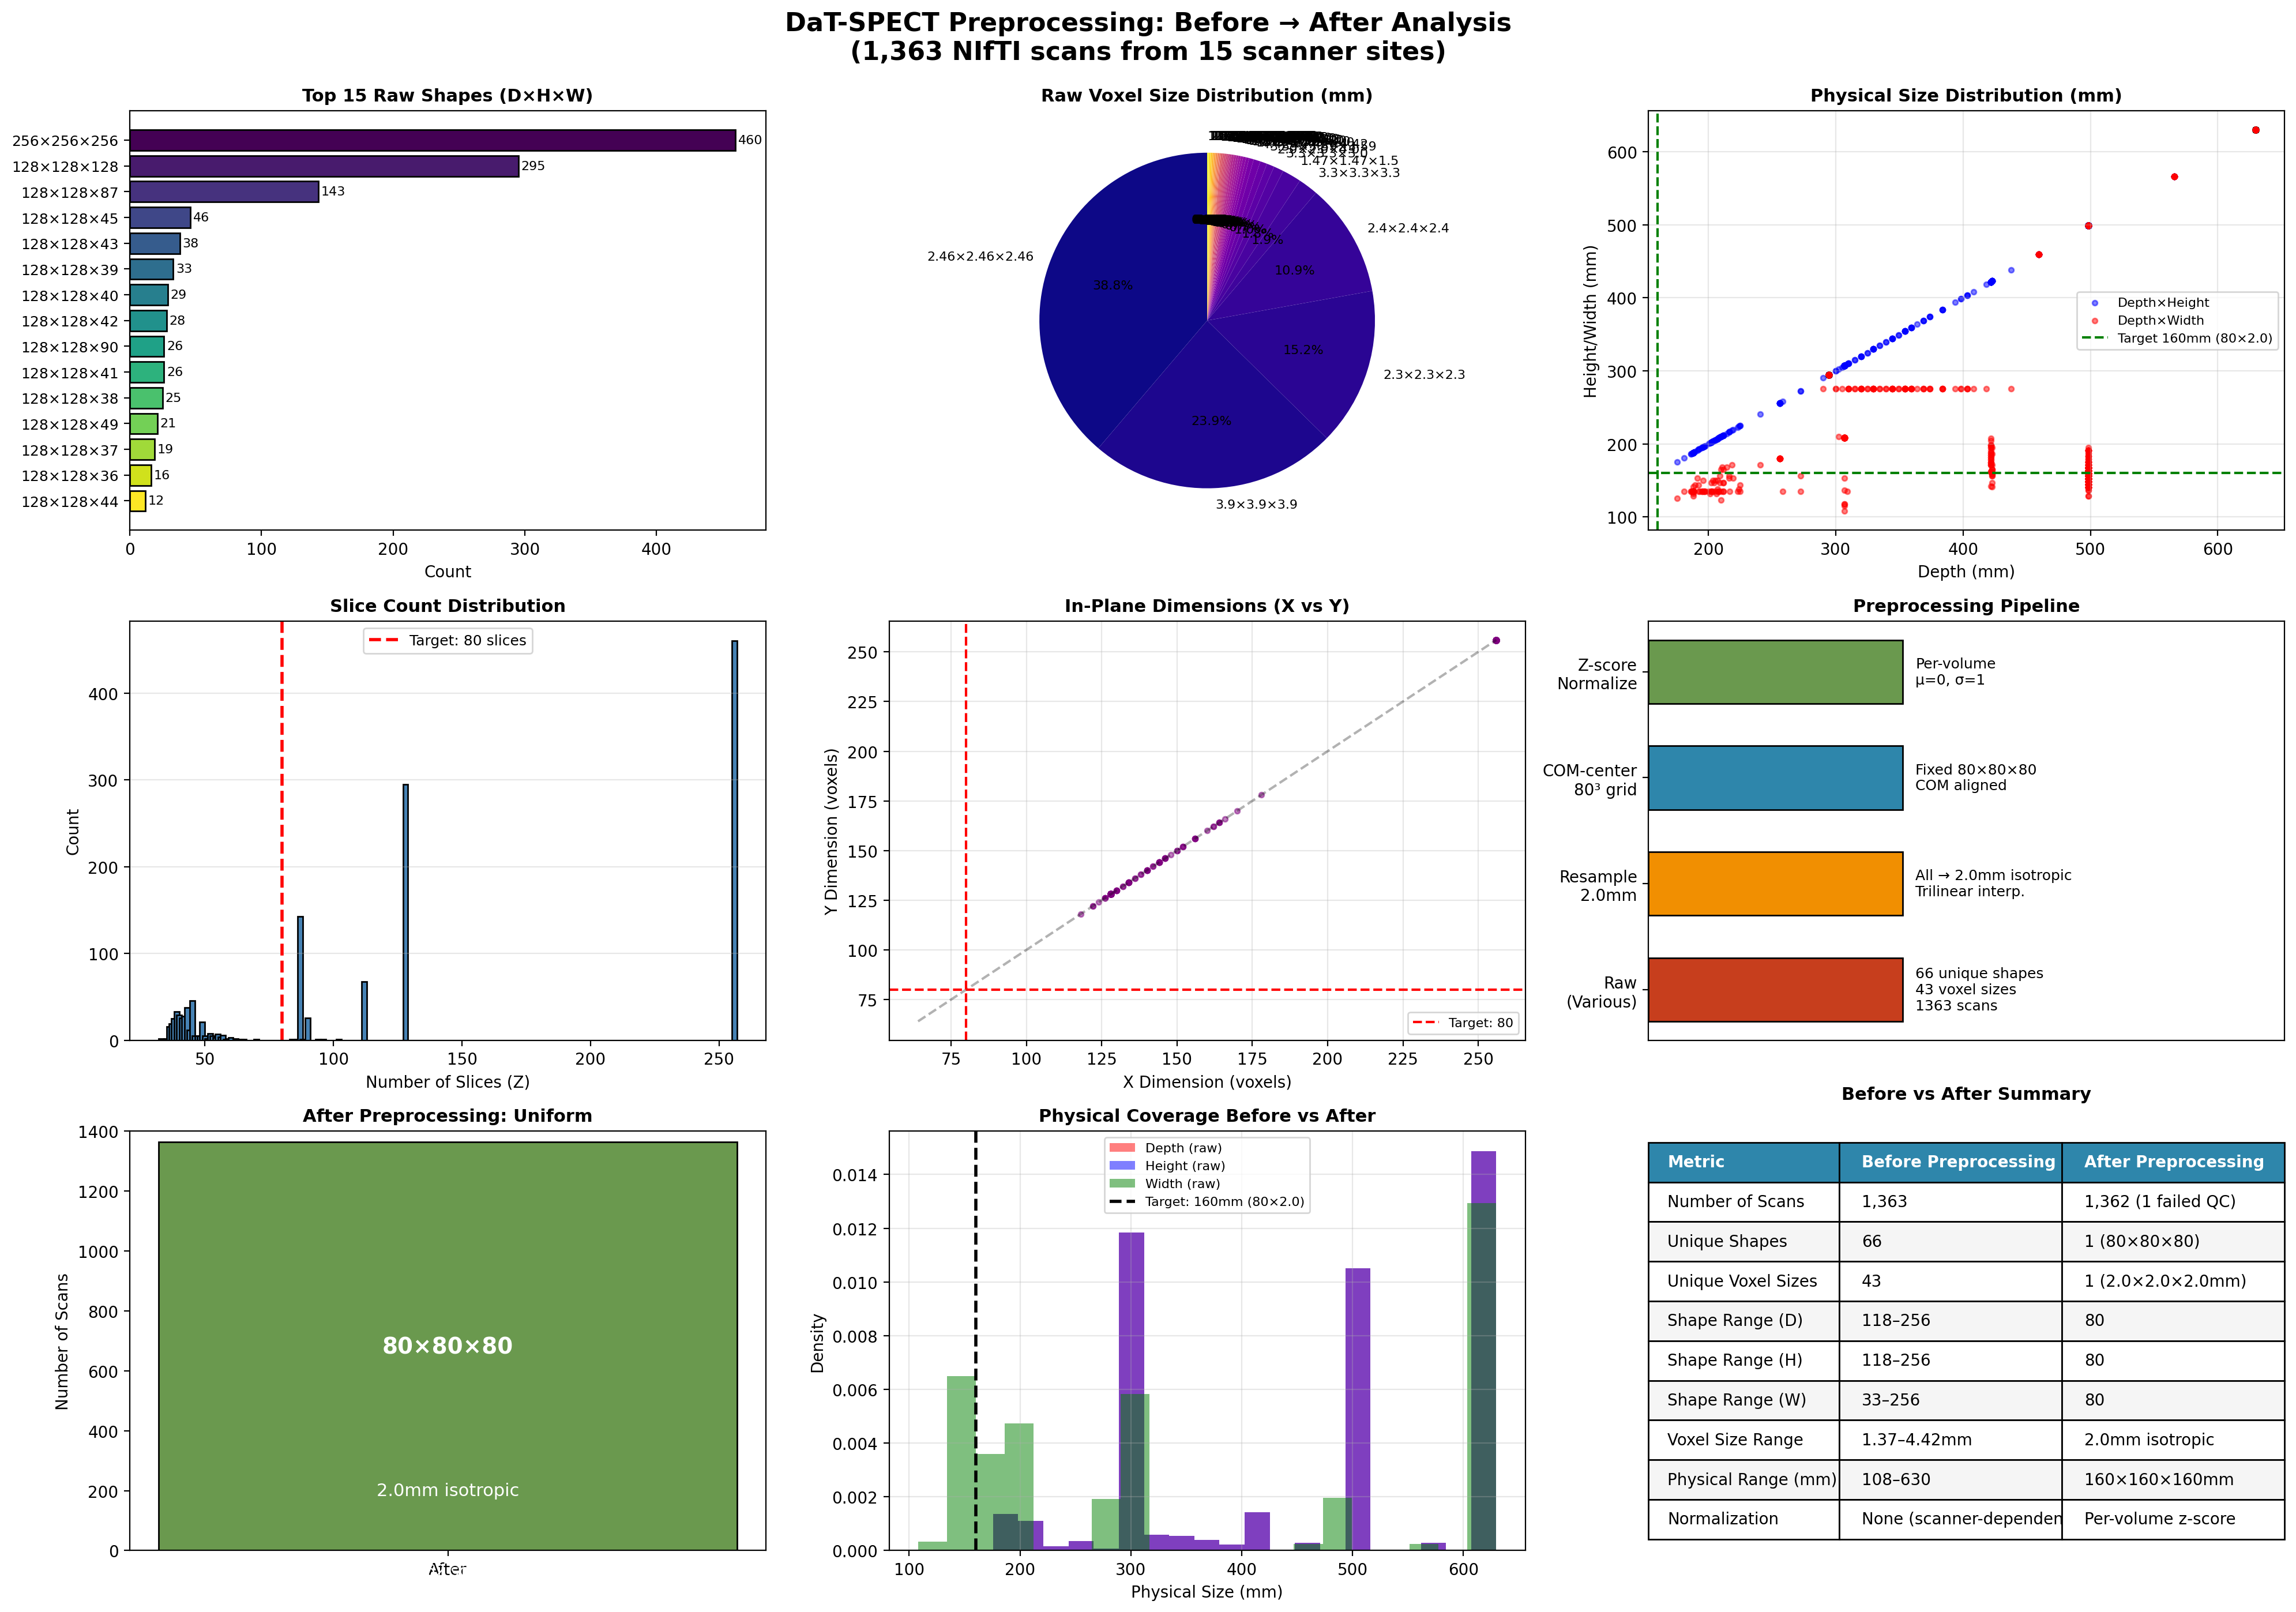
\includegraphics[width=0.98\linewidth]{figures/preprocessing_before_after.png}
    \caption{Multi-site spatial standardization pipeline. (Top) Input heterogeneity across 15 acquisition centers. (Bottom) Standardized isotropic $80^3$ volumetric grids.}
    \label{fig:preprocessing}
\end{figure}

\textbf{Contributions:} To address these challenges, this paper presents a systematic, end-to-end framework for 3D volumetric medical image classification:
\begin{enumerate}
    \item \textbf{Spatial Standardization:} A deterministic preprocessing pipeline enforcing RAS orientation, $2.0~\text{mm}^3$ isotropic resampling, and center-of-mass aligned $80^3$ bounding box cropping.
    \item \textbf{Leakage-Safe Validation:} Empirical quantification of scanner-site data leakage, demonstrating that site-aware Stratified Group K-Fold cross-validation is mandatory for realistic generalization estimates.
    \item \textbf{3D Deep Learning vs. Biomarker Baseline:} A rigorous head-to-head comparison between 3D Deep ResNets and anatomically-guided quantitative ROI biomarkers with Gradient Boosted Trees.
    \item \textbf{Regularization \& TTA:} An ablation of 3D Mixup ($\alpha=0.2$), Label Smoothing ($\epsilon=0.05$), and 15-view Test-Time Augmentation (TTA).
    \item \textbf{Probability Calibration:} Application of post-hoc Platt scaling, reducing Expected Calibration Error (ECE) by 57\% while maintaining peak AUROC ($0.9610$).
\end{enumerate}